\documentclass[manuscript]{aastex}

% load SIUnitX package while avoiding name clash with AASTeX
\usepackage{savesym}
\savesymbol{tablenum}
\usepackage{siunitx}
\restoresymbol{SIX}{tablenum}

% convenient macros every physicist should use
\usepackage{physics}


% title page extras
\slugcomment{An exercise in writing journal articles in {\LaTeX}.}
\shorttitle{Angular momentum at every scale}
\shortauthors{Wysocki and Willard}



\begin{document}

\title{Angular momentum at every scale, \\
       an exercise in circular reasoning}


\author{D. Wysocki}
\affil{
  School of Physics and Astronomy,
  Rochester Institute of Technology,
  Rochester, NY 14623
}
\email{dw2081@rit.edu}

\and

\author{F.D.C. Willard} % not a cat
\affil{
  Physics Department,
  Michigan State University,
  East Lansing, MI 48824
}

\begin{abstract}
Since the works of Newton et al., it has been believed that a correlation exists between an object's mass and angular momentum. Taking a sample of objects on varying scales, and using some circular reasoning, we find the relation $\log{L} = -0.6306 + 1.5810 \log{m}$, with an $R^2$ of $0.993$. Using this relation, we determine the mass of globular cluster 47 Tucanae to be $\SI{3.25e56}{\kilo\gram.\meter^2.\day^{-1}}$, answering a century-old question.
\end{abstract}

\keywords{angular momentum, extrapolation, circular reasoning, science}


\section{Data}

Our data were obtained from Wikipedia et al., and are shown in Table \ref{tab:raw-data}. Just the masses and rotational angular momenta are shown in Table \ref{tab:m-L}. We were able to obtain the mass ($m$), effective radius ($r$), and rotation period ($P$) for each object (with the exception of 47 Tuc and the Milky Way). To determine angular momentum ($L$), we assumed each object to be a sphere, and used
%
\begin{equation}
  \label{eq:angular-momentum}
  L =
  I \omega =
  \qty(\frac{2}{5} m r^2) \qty(\frac{2 \pi}{P}) =
  \frac{4 \pi}{5} \frac{m r^2}{P}.
\end{equation}

For the Milky Way, we cannot assume it to be spherical, and so we took an estimate of the angular momentum from Wikipedia et al., which is based on a more complex model.

\begin{table}[b]
  \centering
  \begin{tabular}{lrrrr}
    \tableline
               & $m (\si{kg})$     & $r (\si{m})$     & $P (\si{d})$   & $L (\si{J s})$     \\
    \tableline
    951 Gaspra & \num{2.5e+16}     & 6100             &  0.293         & \nodata \\
    Ceres      & \num{9.393e+20}   & 473000           &  0.37809       & \nodata \\
    Earth      & \num{5.97237e+24} & \num{6.3781e+06} &  0.99727       & \nodata \\
    Jupiter    & \num{1.8986e+27}  & \num{7.1492e+07} &  0.41007       & \nodata \\
    Sun        & \num{1.98855e+30} & \num{6.9634e+08} & 25.38          & \nodata \\
    Betelgeuse & \num{2.7e+31}     & \num{7.5e+11}    & \num{4.32e+08} & \nodata \\
    47 Tuc     & \num{1.39e+36}    & \num{5.7e+17}    & \nodata        & \nodata \\
    Milky Way  & \num{2.3e+42}     & \nodata          & \nodata        &   1e+67 \\
    \tableline
  \end{tabular}
  \caption{Data obtained from Wikipedia et al.}
  \label{tab:raw-data}
\end{table}

\begin{table}[b]
  \centering
  \begin{tabular}{lrr}
    \tableline
               & $m (\si{kg})$     & $r (\si{m})$        \\
    \tableline
    951 Gaspra & \num{2.5e+16}     &   \num{9.23545e+19} \\
    Ceres      & \num{9.393e+20}   &   \num{1.6168e+28}  \\
    Earth      & \num{5.97237e+24} &   \num{7.08668e+33} \\
    Jupiter    & \num{1.8986e+27}  &   \num{6.88361e+38} \\
    Sun        & \num{1.98855e+30} &   \num{1.10513e+42} \\
    Betelgeuse & \num{2.7e+31}     &   \num{1.02265e+42} \\
    47 Tuc     & \num{1.39e+36}    &   \nodata           \\
    Milky Way  & \num{2.3e+42}     &   \num{1e+67}       \\
    \tableline
  \end{tabular}
  \caption{Mass and angular momenta calculated from Wikipedia et al. data.}
  \label{tab:m-L}
\end{table}

\begin{figure}[b]
  \centering
  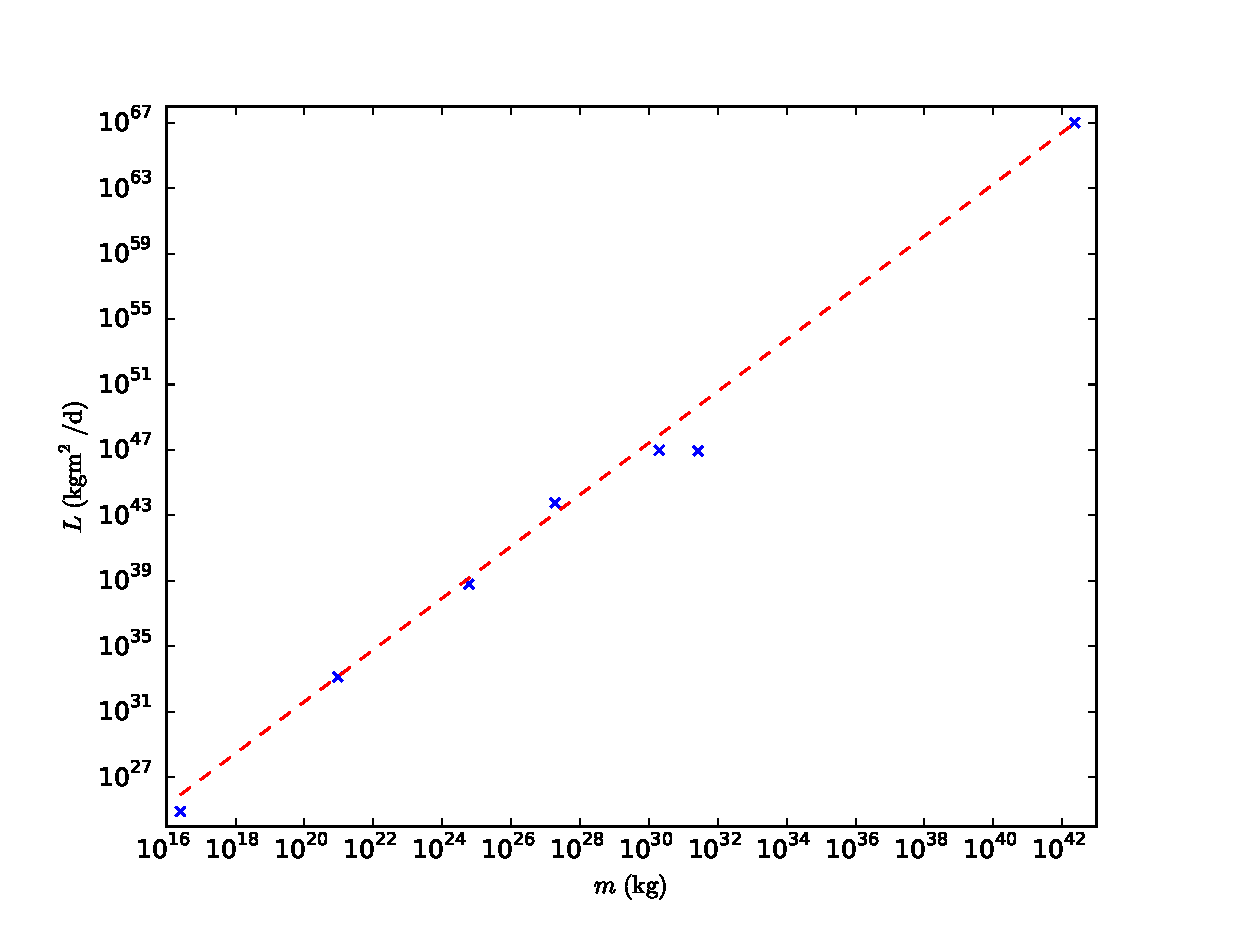
\includegraphics[width=0.85\textwidth]{m-L_log-log}
  \caption{$\log$--$\log$ plot of angular momentum as a function of mass.}
  \label{fig:m-L-log-log}
\end{figure}


\section{Analysis}

We fit a linear model to the mass and angular momenta in log-space, finding a relation of
%
\begin{equation}
  \log L = -0.6306 + 1.5810 \log m,
  \label{eq:log-log-relation}
\end{equation}
%
with an $R^2 = 0.993$, and $F$-statistic of $722.1$. If we return from log-space, we get a relationship of
%
\begin{equation}
  L = 0.234 m^{1.5810}.
  \label{eq:normal-relation}
\end{equation}
%
A $\log$--$\log$ plot of the angular momenta as a function of mass are given in Figure \ref{fig:m-L-log-log}.


Using this relation, we determine the angular momentum of 47 Tucanae to be $\SI{3.25e56}{\kilo\gram.\meter^2.\day^{-1}}$.



\section{Conclusions}

We find that $\log$--$\log$ plots are the ``bread and butter'' of astronomical publications. However, we hypothesize that one's academic career cannot survive on bread and butter alone.


\acknowledgments

The authors are thankful of our sponsors: National Science Flounder grant 1234, and National Acrobatics and Space Administration grant 5678. F.W. would Jack Hetherington for all the tuna. We are grateful for the helpful feedback from the referee.


\end{document}
